
\section{Development Process}

Given the iterative nature of our work schedule and of the meeting
with our customer, as well as his request for intermediate prototypes
to be presented during these meetings, the choice of Scrum as a development
process was natural. Moreover, everybody in the team had previous
experiences with Scrum from earlier projects. With our choice of Scrum
as process development model, we set up some guidelines for ourselves
so that we could follow the intended process as closely as our task
and experience allow. To do we have adopted some changes in the process.


\subsection{Modifications to our project}

To make it more suitable to our schedule we made some slight modifications
to the Scrum model. The meetings will be held three times a week (on
Monday, Wednesday and Friday) and we will have work sessions on these
days too. Sprints will be modified to be primarly bi-weekly, but time
between Sprints may vary depending on the priorities identified during
the meetings with the customer and the risk analysis. Sprint backlogs
will be very crucial in this regard. With the abstract goals of the
project set forth, the gradual inclusion of new features as we and
the customer see the project evolve will be mirrored in the backlogs
from sprint to sprint. We will also maintain a product backlog with
feedback provided by the customer. To better fit our product goals
the differences between faculties of a normal product backlog and
the requirements and wishes of the customer we will have to modify
the backlog to be somewhat of an intersection between requirements
and feature goals. Another important difference to normal Scrum evolution
will have to be the “definitions of done”. As our end state is diffuse
in regards to the tangible product we have in collaboration with the
customer some design goals(see requirements) that will be the main
focus of our project.


\subsection{Project management tools}

To accompany us in the Scrum process we have chosen an online tool
called ScrumDo (www.scrumdo.com). This tool has features for most
if not all parts of the Scrum process. Using this tool consistently
will be our main method of maintaining and separating packages from
the WBS (Work Breakdown Structure). In the context of ScrumDo and
Scrum these low level work packages are called stories and are moved
accordingly from \char`\"{}ToDo\char`\"{} over to \char`\"{}In progress\char`\"{}
and eventually to \char`\"{}Done'' areas.
	
\begin{figure}[h!]
\centering 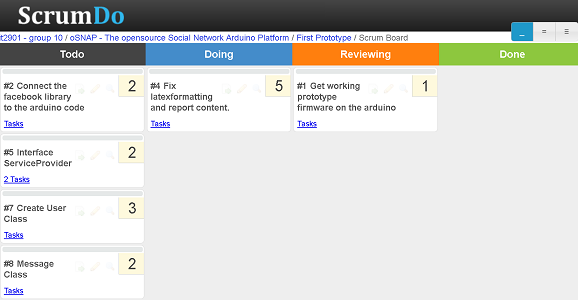
\includegraphics{img/management-scrumdo} \caption{The Scrum Board in ScrumDo}

\label{fig:management-scrumdo}
\end{figure}
	
Another part of the project is the collaboration software.
Initially we decided to use Git which is a fast, scalable,
distributed revision control system with an unusually rich command
set that provides both high-level operations and full access to internals.
It differs from the centralised control systems like SVN for its capability
to handle several software \char`\"{}branches\char`\"{} at once. The
branches can head in different directions and can later be merged
instead of always maintaing a central, \char`\"{}correct\char`\"{}
version. NTNU provided SVN and Trac repositories to keep track of our
project and we will use these to share finished code for evaluation
purposes. We decided to use Git due to its higher flexibility and because
of the experiences the team members already had with it.

\section{Risk analysis and mitigation strategies}
todo: add risk analysis